Este capítulo apresenta um estudo exploratório realizado com o objetivo de verificar a viabilidade e aperfeiçoar a proposta com base nas descobertas e desafios enfrentados durante o processo. Destaca-se que este estudo teve o foco apenas na análise das avaliações de acessibilidade e não explorou as sugestões de modificações e as alterações realizadas no código das aplicações. Todas as decisões de projeto e metodologia adotada estão em conformidade com o que foi descrito no Capítulo~\ref{chap:proposta}.
Além disso, também são descritas as atividades já realizadas do cronograma proposto.

\section{Questões de pesquisa}

As seguintes questões de pesquisa foram definidas para este estudo exploratório:
\begin{itemize}
 \item RQ1 - Quantas avaliações de usuário são relacionadas a acessibilidade e qual é a sua distribuição? 
 \item RQ2 - Qual é a diversidade de tópicos de acessibilidade abordados nas avaliações dos usuários?
 \item RQ3 - Quais são as notas associadas às avaliações que abordam aspectos de acessibilidade?  
\end{itemize}

\section{Seleção de aplicativos móveis}

Os critérios de seleção dos aplicativos para este estudo seguem os critérios definidos na Seção~\ref{sec:selecao}. Portanto, foram selecionadas aplicações da plataforma Android que satisfaziam as seguintes condições: estavam disponíveis na Google Play Store e o código-fonte estava armazenado em um repositório público da plataforma GitHub. Ao todo, apenas 701 aplicativos dentre os mais de 2000  indexados no FDroid\footnote{Dados de julho/2019} satisfizeram esses critérios.

A Tabela~\ref{tab:summarygps} mostra a distribuição de alguns atributos dos aplicativos selecionados por meio de estatística descritiva utilizando o resumo dos cinco números (mínimo amostral, quartil inferior, 
mediana, quartil superior, máximo amostral), a média e o desvio padrão. 
A maioria dos aplicativos tem até 9 atividades, mas há aplicativos muito maiores, como o ``Slide for Reddit'', por exemplo, que possui 91 atividades.

\begin{table}[htb]
%\setlength{\tabcolsep}{0pt}

\centering
\caption{Statistics on the Google Play Store sample}
\small
\label{tab:summarygps}
\begin{tabular}{lrrrrr}
\hline
             & Atividades & Nota & Avaliações     & Instalações  & Comentários \\
\hline
Mínimo          & 1          & 0     & 0            & 0         & 0       \\
Quartil Inferior           & 2          & 4           & 50    & 1K      & 4       \\
Mediana       & 5          & 4.3   & 130         & 10K     & 22      \\
Quartil Superior          & 9          & 4.6   & 836        & 50K     & 145     \\
Máximo          & 92         & 5     & 3.6M    & 100M & 4480    \\
Média         & 8.16       & 4.16  & 12.4K     & 550K+    & 305.4   \\
Desvio Padrão        & 10.5       & 0.79  & 151.6K  & 5.7M   & 840.8  \\
\hline
\end{tabular}
\end{table}

A maioria dos aplicativos possui uma boa nota e a maioria foi avaliada por até 836 usuários. O número de avaliações apresentado na tabela é diferente do número de comentários, pois quando um usuário faz uma avaliação ele é obrigado a atribuir uma nota, mas não é obrigado a inserir um comentário. Existem aplicativos que possuem um número muito alto de avaliações, como o Telegram, que possui 3,6 milhões de avaliações. O Telegram também é o aplicativo mais instalado (100 milhoes de istalações).
Por outro lado, o número de comentários não é muito alto, pois a maioria dos aplicativos recebeu até no máxmio 145 comentários em suas avaliações. O número máximo de revisões desta amostra é de 4480 em razão das limitações da API utilizada. Esta limitação não teve muito impacto neste estudo exploratório porque apenas 15 aplicativos (2\%) possuem mais de 4480 revisões registradas na Google Play Store.


\section{Extração e seleção das avaliações}

Uma aplicação escrita na linguagem Python foi escrita para consumir os dados da Google Play Store utilizando a API \emph{google-play-api}\footnote{https://github.com/facundoolano/google-play-api}. Como mencionado anteriormente, na versão utilizada, esta API só permite o retorno de no máximo 4480 avaliações de cada aplicativo. Além disso, só foram recuperadas avaliações escritas em inglês, que é o idioma padrão definido pela API.


A seleção das avaliações que possivelmente estão relacionadas a algum aspecto de acessibilidade da aplicação foi feita por meio da utilização de palavras-chave aplicadas aos comentários dos usuários. 
Para isso, um conjunto de palavras-chave foi definido com base nas diretrizes de acessibilidade da BBC~\cite{bbc}. Este guia de acessibilidade possui 54 recomendações que são classificadas em onze diferentes categorias: áudio e vídeo (5); design (12); editorial (3); foco (6); formulários (6); imagens (2); links (3); notificações (4); scripts e conteúdo dinâmico (4); estrutura (4); e texto equivalente (5). 
Este padrão foi selecionado porque ele tem o foco em aplicações móveis e possui exemplos de implementação e de teste de cada recomendação, o que permite compreender melhor os tipos de problemas de acessibilidade tratados no guia. 

Foram definidas 213 palavras-chave com base na análise de cada recomendação do guia. 
A Tabela~{tab:keywords} mostra exemplos das palalavras-chave utilizadas.
Note que foram utilizadas variantes das palavras (exemplo: \textit{cannot see} e \textit{can't see}, ou \textit{color} e \textit{colour}, ou \textit{impaired} e \textit{impairement}) para garantir que nenhuma avaliação relevante fosse excluída. Infelizmente, não é possível capturar casos em que as palavras foram escritas com a grafia errada. A lista completa das palavras-chave podem ser vistas em um repositório criado para armazenar dos dados deste estudo\footnote{https://github.com/marceloeler/data-ihc2019}.


\begin{table}[!htb]
\small
\caption{Exemplos de palavras-chave utilizadas para selecionar avaliações relacionadas à acessibilidade das aplicações}
\label{tab:keywords}
\begin{tabular}{|l|l|}
\hline
Categorias & Palavras-chave \\
\hline
Gerais                    & accessibility, disability, screen reader, Talkback, operable, impaired, 
\\& impairment                                               \\

\hline
Áudio/Vídeo             & subtitle, sign language, audio description,
 transcript, autoplay, mute, \\& volume                                                 \\

\hline
Design                      & contrast, background color, blind, flicker,
 visual cue, touch size, \\&overlap, font size, 
 dark/light mode, eyestrain, seizure, can't see \\

\hline
Editorial                   & consist. label, language, visual/audio cue                                                                \\

\hline
Foco                       & focusable, control focus, keyboard trap, 
 focus order, navigable                        \\

\hline
Formulários                       & unique label, missing label, content description,
 input type, \\& input format, focusable                                                                        \\

\hline
Imagens                      & image of text, hidden text, text alternative,
background image                                                                                               \\

\hline
Links                       & link description, unique desc., duplicate
link, alternative format \\

\hline
Notificações               & inclusive, haptic, vibration, feedback, alert 
 dialog, understandable, \\& unfamiliar                                                                             \\

\hline
Conteúdo dinâmico & animated content, page refresh, automatic  
refresh, timeout,  adaptable, \\&input sign                                                               \\

\hline
Estrutura                   & page title, screen title, heading, header                                                                                                         \\
\hline
Texto equivalente             & alternative text, non-visual, blind, screen reader, content description  \\
\hline
\end{tabular}
\end{table}

O uso de palavras-chave pode trazer muitos falsos positivos, uma vez que várias palavras utilizadas podem ter conotações diferentes em diferentes contextos. Por isso foi realizada uma análise manual de todas as avaliações que possuíam pelo menos uma palavra-chave definida. Neste estudo, apenas uma pessoa fez a análise manual das avaliações. Além disso, as avaliações não selecionadas por palavras-chave não foram analisadas para saber se alguma delas não foi selecionada pela ausência de alguma palavra-chave relevante e que não foi utilizada. Durante a análise manual, as avaliações confirmadas também foram classificadas em: 
requisições, quando o usuário reporta algum problema de acessibilidade ou solicita alguma modificação ou adição para tornar a aplicação mais acessível;
ou elogios, quando o usuário parabeniza o aplicativo pelo seu nível de acessibilidade.


\section{Análise dos resultados}

As avaliações selecionadas com base nas palavras-chave e na validação manual foram analisadas para responder as questões de pesquisa propostas no estudo exploratório. A seguir as respostas às questões de pesquisa são apresentadas em detalhes. 

 
\subsection{RQ1 - Quantas avaliações de usuário são relacionadas a acessibilidade e qual é a sua distribuição? }

No total, foram extraídas 214.053 avaliações completas (com nota e comentário) dos 701 aplicativos da amostra. 
Dessas avaliações, apenas 5.076 foram pré-selecionadas por meio das palavras-chave. 
Após a análise manual, o número de avaliações de fato relacionadas à acessibilidade das aplicações foi de 2.663. Dos 701 aplicativos da amostra, apenas 276 possuem pelo menos uma avaliação relacionada a acessibilidade.

As 2.663 avaliações de acessibilidade representam apenas 1.24\% de todas as avaliações completas extraídas. A Figura~\ref{fig:distribution-proportion} mostra a distribuição da proporção entre as avaliações de acessibilidade e o número total de avaliações completas de cada aplicativo.
No geral, as avaliações de acessibilidade representam menos de 4\% de todas as reviões feitas para cada aplicativo. Para metade dos aplicativos, elas representam menos de 1.5\%.
Para uma pequena proporção de aplicativos, as avaliações de acessibilidade representam entre 4\% e 9\% das avaliações recebidas. Existem alguns aplicativos para os quais essa proporção varia entre 10\% e 16\%.
Há alguns casos em que o número de avaliações completas é tão pequeno que uma simples avaliação de acessibilidade representa uma grande proporção, como é o caso do aplicativo MuPDF mini, Booky McBookface, e GameDealz, cujas proporções são de 50\% (1/2), 40\% (2/5) e 33\% (1/3), respectivamente.

 \begin{figure}[!htb]
 \centering
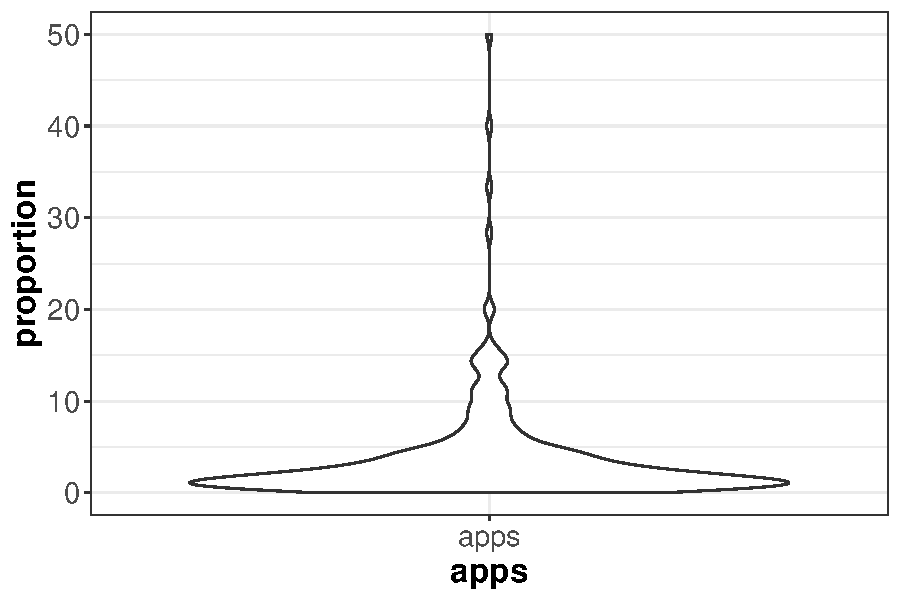
\includegraphics[scale=0.8]{imagens/distribution-proportion-accreviews}
\caption{Distribuição da proporção entre avaliações de acessibilidade e o total de avaliações de cada aplicativo}
\label{fig:distribution-proportion}
\end{figure}



The accessibility reviews are not equally distributed through the 701 apps of our sample.
Only around 40\% of our sample (276 apps) have at least one accessibility review.
It is noticeable that these 276 apps concentrate 92\% (197,419) of all reviews of the sample,
which implies that the more the number of reviews, the more the possibility of receiving accessibility reviews. 
In fact, the Spearman correlation between the number of reviews and the number of reviews related to accessibility is 0.73, which is a strong correlation.

The accessibility reviews are not equally distributed not even through the 276 apps that have accessibility reviews. 
Nearly 65\% (1,745) of the accessibility reviews are concentrated in 35 outliers,
where three apps have more than 100 accessibility reviews (140, 163 and 206) each one while the remaining 32 apps have between 19 and 79 reviews each. 
\autoref{fig:distributionreviewsapp} shows the distribution of accessibility reviews through the 276 apps of our sample. 
The outliers are not represented in this chart to improve its legibility. 
This chart shows that 75\% of the apps have less than 9 reviews, and half of them have up to three accessibility reviews.


\begin{figure}[!htb]
\centering
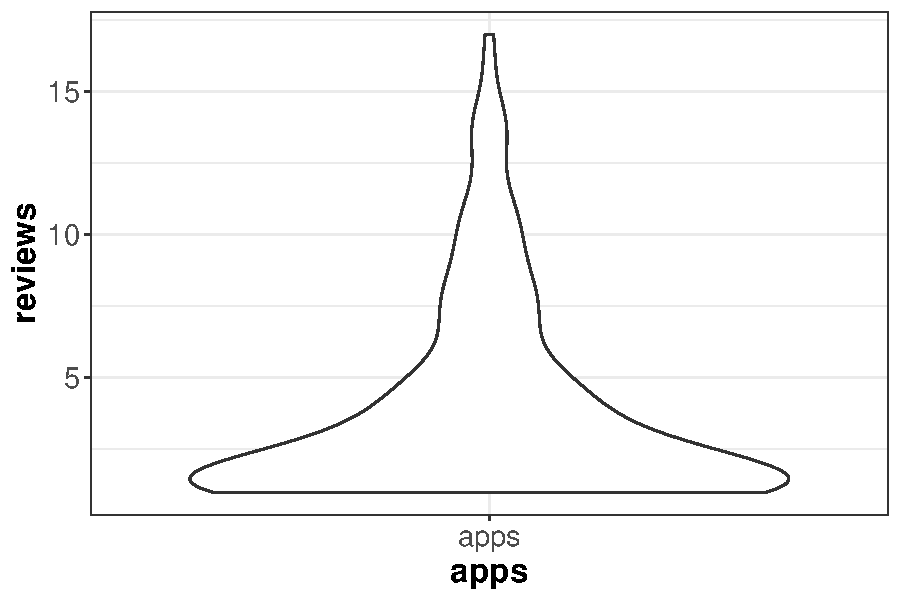
\includegraphics[scale=0.80]{imagens/distribution-accreviews-no-outlier-violin.pdf}
\caption{Distribution of accessibility reviews}
\label{fig:distributionreviewsapp}
\end{figure}


\subsection{RQ2 - Qual é a diversidade de tópicos de acessibilidade abordados nas avaliações dos usuários?}


\begin{table*}[!htb]
\centering
\caption{Number of accessibility reviews by keyword}
\label{tab:keywords-reviews}
\begin{tabular}{lrr||lrr||lrr}
\hline
keyword          & reviews & apps & keyword          & reviews & apps & keyword            & reviews & apps \\
\hline
dark mode        & 645     & 128  & metadata         & 20      & 12   & grouped            & 3       & 3    \\
zoom             & 491     & 80   & too bright       & 20      & 8    & seizures           & 3       & 1    \\
customization    & 309     & 50   & haptic           & 16      & 10   & select language    & 3       & 3    \\
font size        & 214     & 74   & scaling          & 16      & 11   & understandable     & 3       & 3    \\
volume           & 146     & 40   & control key      & 15      & 5    & vibration feedback & 3       & 3    \\
cannot see       & 128     & 57   & voice command    & 14      & 10   & actionable         & 2       & 1    \\
accessibility    & 74      & 44   & text-to-speech   & 13      & 9    & audio cue          & 2       & 2    \\
readable         & 72      & 47   & eyestrain        & 12      & 9    & missing label      & 2       & 2    \\
change font      & 68      & 44   & strain           & 12      & 9    & navigable          & 2       & 2    \\
hard to see      & 58      & 41   & background image & 11      & 8    & verbose            & 2       & 2    \\
background color & 50      & 30   & screen reader    & 11      & 10   & captcha            & 2       & 2    \\
light mode       & 42      & 27   & change language  & 10      & 8    & audio description  & 1       & 1    \\
mute             & 42      & 25   & small widget     & 10      & 9    & container          & 1       & 1    \\
contrast         & 40      & 31   & stop button      & 10      & 5    & distinguishable    & 1       & 1    \\
subtitle         & 40      & 7    & impaired         & 9       & 9    & input type         & 1       & 1    \\
adjustable       & 34      & 23   & text reflow      & 9       & 3    & keyboard language  & 1       & 1    \\
blind            & 31      & 24   & timeout          & 9       & 7    & page refresh       & 1       & 1    \\
header           & 31      & 22   & consistency      & 7       & 7    & page title         & 1       & 1    \\
overlap          & 31      & 25   & epilepsy         & 7       & 1    & sign language      & 1       & 1    \\
pause button     & 27      & 17   & assistance       & 6       & 5    & svg image          & 1       & 1    \\
flicker          & 26      & 19   & colour coding    & 5       & 5    & switch device      & 1       & 1    \\
spacing          & 26      & 17   & transcript       & 5       & 5    & touch target       & 1       & 1    \\
migraine         & 25      & 3    & default language & 4       & 4    & adjust size        & 1       & 1    \\
input method     & 23      & 11   & older device     & 4       & 3    & adjust colour      & 1       & 1    \\
autoplay         & 21      & 17   & visual cue       & 4       & 4    &                    &         &     \\
\hline
\end{tabular}
\end{table*}


The aim of this research question is to understand whether users tend to address only specific issues or a wide range of features related to accessibility. \autoref{tab:keywords-reviews} shows the number of accessibility reviews and apps associated with each keyword we used in our investigation. We only show keywords for which at least one accessibility review was found. We collapsed many keywords (e.g. can't read and cannot read, dark theme and dark mode) for the sake of presentation. 


Clearly, accessibility reviews are concentrated on a small set of keywords. Only six keywords are mentioned in more than 100 accessibility reviews each. The most popular keywords are also mentioned in the reviews of several distinct apps. For instance, the keywords associated with ``dark mode'' appears on 628 accessibility reviews and 128 distinct apps, which is almost half of the apps with accessibility reviews. 


%can't see -> cannot see
%difficult to see -> hard to see
%difficult to read -> hard to see
%can't read -> cannot read
%cannot read -> cannot see
%impossible to see -> cannot see
%impossible to read -> cannot see
%dark theme -> dark mode
%night theme -> dark mode
%night mode -> dark mode
%black theme -> dark mode
%black mode -> dark mode
%text size -> font size
%accessible -> accessibility
%background colour -> background color
%adjust font -> change font
%text resize -> change font
%headache -> migraine
%auto-play -> autoplay
%play automatic -> autoplay
%strain -> eyestrain
%tiny font -> small font
%larger font -> change font
%heading -> header
%white mode -> light mode
%light theme -> light mode
%white theme -> light mode
%personalization -> customization
%magnify -> zoom
%screenreader -> screen reader
%impairment -> impaired
%disabled person -> impaired
%adaptable -> adjustable
%tooltip -> assistance
%font sizing -> change font
%no label -> missing label
%large font -> change font
%small font -> change font
%talkback -> screen reader
%small button -> small size
%overlap -> spacing

Solely analysing the frequency of keywords in accessibility reviews is not enough to understand the diversity of features addressed by user reviews. 
Many keywords are associated with the same accessibility feature or issue. 
For instance, the keywords dark mode, night mode and black mode belongs to the same accessibility aspect: dark mode. 
Therefore, we grouped several keywords to represent a single accessibility topic and to make it easy to analyse the results.
%Moreover, the keyword itself does not evidence to which specific problem the user is referring to. Manual validation helped to make it clear that only reviews related to an accessibility issue or compliment were selected, but in this study we did not specify what was the problem. 


\begin{table}[]
\centering
\caption{Number of distinct apps and reviews by grouped features related to accessibility}
\small
\label{tab:group-keywords}
\begin{tabular}{lrrrr}
\hline
Topic         & Reviews & \% (Reviews) & Apps & \% (Apps) \\
\hline
Theme/Mode    & 726     & 27\%     & 144  & 52\%  \\
Zoom          & 506     & 19,0\%     & 83   & 30,1\%  \\
Customization & 351     & 13\%     & 63   & 23\%  \\
Media         & 309     & 11,6\%     & 82   & 29,7\%  \\
Font          & 249     & 9,4\%      & 83   & 30,1\%  \\
Contrast      & 218     & 8\%        & 91  & 33\%  \\
Impairment    & 135     & 5,1\%      & 70   & 25,4\%  \\
Flickering    & 87      & 3,3\%      & 31   & 11,2\%  \\
Accessibility & 74      & 2,8\%      & 44   & 15,9\%  \\
Size          & 66      & 2,5\%      & 45   & 16,3\%  \\
Input alternatives        & 54      & 2,0\%      & 25   & 9,1\%   \\
Feedback      & 19      & 0,7\%      & 11   & 4,0\%   \\
Language      & 15      & 0,6\%      & 11   & 4,0\%  \\
\hline
\end{tabular}
\end{table}

\autoref{tab:group-keywords} shows the accessibility topics (Column 1), the number of distinct reviews related to that topic (Column 2), the proportion between the number of reviews and the total number of accessibility reviews (Column 3), the number of distinct apps covered by that topic (Column 4), and the proportion between the number of distinct apps and the total number of apps with accessibility reviews (Column 5).
We did not use the general guidelines of the BBC standard as accessibility topics because they are coarse grained groups. In that case, most topics or features would fall into the Design guidelines group.


Theme/Mode is the most popular topic among user reviews.
It aggregates all accessibility reviews that contain keywords related to colour modes and themes. Around 27\% of the accessibility reviews are associated with this specific topic, and nearly half of the apps received at least one review within this topic.
The second most popular topic is related to zooming features, which have almost 20\% of the accessibility reviews and are associated with the reviews of 30\% of the apps.

Many users request features that enable font and specially font size adjustments. This topic represents almost 10\% of the accessibility reviews and are related to 30\% of the apps.
Although theme/mode and font size adjustments are features linked to the customization of the app, we created a specific topic to show how many reviews explicitly mention customization features. 

Media and dynamic content control (volume control, pause button, stop button, autoplay, etc) are also within the most popular accessibility topics. It is related to nearly 12\% of the accessibility reviews and 82 apps (30\%). 
The poor contrast between elements of the foreground and the background make text and visual components difficult to see or read. Most user complaints associated with the keywords ``cannot see'', ``hard to see'', and many others are related to poor contrast. Contrast issues are reported in 8\% of the accessibility reviews and 33\% of the apps.

Accessibility reviews that directly address user's disabilities or aspects of the user interface that can specially impact disabled users are not too popular, but represent 5\% of the accessibility reviews and cover 70 apps (25\%). The keywords accessibility and accessible were mentioned in only 3\% of the reviews and for a small number of apps (16\%).
The remaining topics, although important for what accessibility is concerned, are not frequent among user reviews.

We also analysed the diversity of accessibility reviews for each individual app to check whether users reported more than one type of issue by app.
To do so, we analysed how many keywords and accessibility topics were mentioned in the accessibility reviews of each app. 
\autoref{fig:distributiontopicsapps} shows the distribution of the number of keywords mentioned in the accessibility reviews of each app (left side). 
For most apps, the accessibility reviews are related to six keywords at most. For half of the apps, this number is reduced to three. Few apps have more than 15 keywords on their accessibility reviews. The Cool Reader app is one of the outliers of the group for it received accessibility reviews containing 36 distinct keywords. As most apps have few accessibility reviews, the diversity of keywords mentioned in accessibility reviews is poor. In fact, the Spearman correlation between the number of keywords and the number of reviews is 0.93, which might imply that the more the number of reviews, the more the diversity of reviews.


 \begin{figure}[!htb]
 \centering
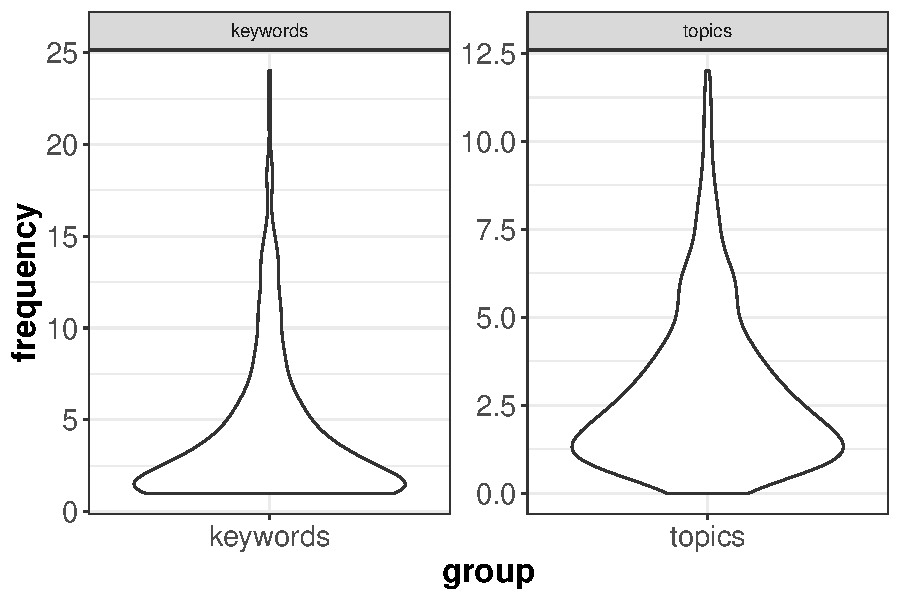
\includegraphics[scale=0.8]{imagens/distribution-topics-keywords.pdf}
\caption{Distribution of accessibility topics and keywords through the accessibility reviews of each app}
\label{fig:distributiontopicsapps}
\end{figure}


\autoref{fig:distributiontopicsapps} shows the distribution of the number of accessibility topics mentioned in the accessibility reviews of each app (right side). The fact that the accessibility reviews of an app contains several keywords does not necessarily mean the reviews are diverse for many keywords are related to the same issue or accessibility aspect. Notice that the accessibility reviews are concentrated in two to four accessibility aspects while some apps have accessibility reviews related to almost all accessibility concerns we mentioned. The app Calculator,
%\footnote{https://play.google.com/store/apps/details?id=com.android2.calculator3}, 
for example, have accessibility reviews that address 12 of the accessibility topics presented in~\autoref{tab:group-keywords}. Although the Spearman correlation between the number of reviews and the number of topics is strong (0.87), this app has only 60 accessibility reviews. The next most diverse app with respect to accessibility reviews are the Cool Reader app and the Hacker's Keyboard, %\footnote{https://play.google.com/store/apps/details?id=org.coolreader}
with 11 accessibility topics each app.




\begin{comment}

We grouped the number of accessibility reviews based on the accessibility guidelines we used to define the keywords~\cite{bbc}. \autoref{tab:guideline-reviews} shows the number of accessibility reviews we found by each guideline. As for the keywords, some accessibility aspects may be related to more than one guideline. The design guideline is by far the most relevant feature in this context since around 79\% of the accessibility reviews refer to it. This is not surprising once the design guideline cover most aspects of the user interface, such as colour choices, widget sizes, font/color/size/content adjustments, spacing, focus, and so forth. The second most relevant guideline is related to Audio and Video, which covers alternatives for audio and visual content, automatic play, metadata, volume control and audio conflict. The remaining guidelines are rarely mentioned by users on their reviews.

\begin{table}[!htb]
\caption{Number of accessibility reviews by accessibility guideline}
\label{tab:guidelines-reviews}
\begin{tabular}{lrr}
\hline
Guideline        & Reviews & Proportion   \\
\hline
Audio/video      & 303     & 10\% \\
Design           & 2369    & 79\% \\
Editorial        & 17      & 1\%  \\
Focus            & 67      & 2\%  \\
Forms            & 19      & 1\%  \\
Images           & 23      & 1\%  \\
Links            & 0       & 0\%  \\
Notifications    & 21      & 1\%  \\
Dynamic content  & 85      & 3\%  \\
Structure        & 14      & 0\%  \\
Text equivalents & 67      & 2\% \\
\hline
\end{tabular}
\end{table}


As the BBC accessibility guidelines can cover a wide range of accessibility features, we grouped the accessibility reviews by specific issues to understand the most relevant aspects of apps usability. The most mentioned feature in this context is the Adjustability (under the Design guideline) feature. Almost 1300 reviews mention features related to the adaptation of the user interface. By far, the most requested feature is to change colour themes or modes, in which users can choose between blind, dark, night, light, white mode, for instance. The second most requested features is the capacity to change the text, contrast and content size (nearly 600 reviews). Content resizing (e.g. zooming) is also a feature commonly requested by users (488 reviews).

Media control (e.g. pause and stop button, mute, volume control, subtitle) is also a frequent requested features. In many reviews, users also mention they cannot perceive (e.g. keywords cannot see, impossible to see) all elements of the user interface due to several reasons: low contrast ratio, bad colour choices, small fonts and widgets, and so forth. Around 250 reviews mention this problem. Few reviews address issues directly associated with disabled users, where blind users and assistive technologies are mentioned. Some reviews also report flickering screens that may cause migraine, headache and even seizures to epileptic users.\\
\end{comment}

\subsection{RQ3 - Quais são as notas associadas às avaliações que abordam aspectos de acessibilidade?}


Not all reviews have features requests or bug reports. Many users give positive feedback on the apps they like. 
During our analysis, a review was marked as a compliment when a positive feedback was given on some accessibility aspect of the app. 
For instance, the review \textit{``I am totally blind - and Cool Mic is fully compatible with Android's built in TalkBack screenreader. Great work guys!''} is a positive feedback.
In our sample, around 76\% (2018) of the accessibility reviews are requests or complaints, and 24\% (645) are compliments. 
The 645 positive feedback on accessibility are distributed over 110 apps, while the requests/complaints reviews are distributed over 262 apps. There are 166 mobile apps that received only requests/complaints and 14 mobile apps that received only compliments.

One of the purposes of this research question is to find out whether users give a bad score when make a request related to accessibility and a good score when praise the app for its accessibility. 
\autoref{fig:reqcompscores} shows a violin plot to compare the scores obtained for these two samples. Surprisingly, it seems there is no significant difference between these two groups. 

 \begin{figure}[!htb]
 \centering
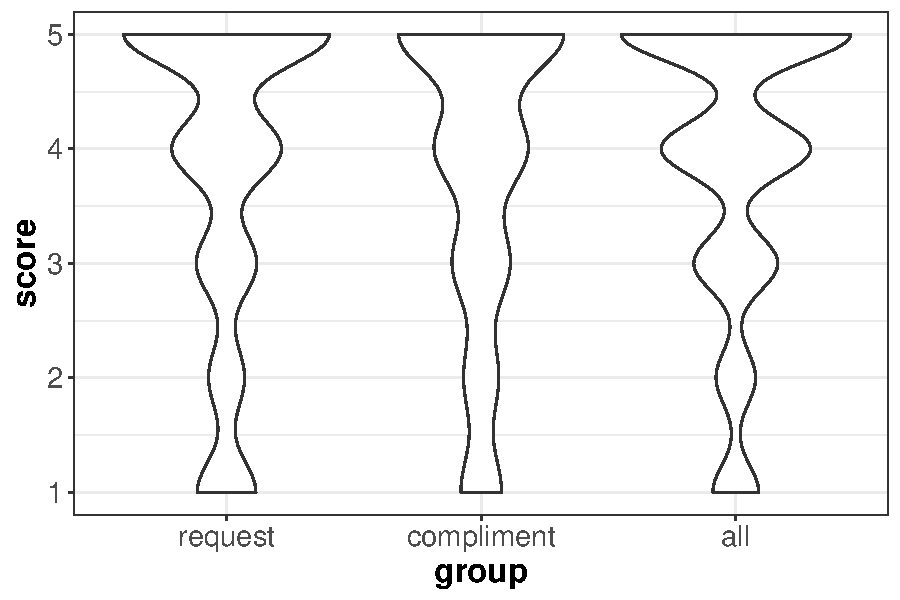
\includegraphics[scale=0.8]{imagens/scores-compliment-request.pdf}
\caption{Comparison between the scores associated with request and compliment reviews}
\label{fig:reqcompscores}
\end{figure}

In addition, we want to know whether reviews associated with different topics or keywords present lower or greater scores. 
\autoref{fig:scoresthemes} shows a violin plot to compare the scores of reviews related to specific accessibility topics (cf. \autoref{tab:group-keywords}). In this case, we only plotted data from reviews that contain accessibility requests or complaints. For some accessibility topics, even though users requested features that can make the mobile app more accessible, scores are concentrated in 4 or 5. This is the case of topics such as, for example, ``customization'', ``font'', ``media'', ``size'' and ``theme''. For other topics, it is clear that the reviews scores are concentrated between 2 and 4. The concentration of scores below 3 related to the keywords ``contrast'', ``flickering'' and ``zoom'' indicates that users are more affect by those issues than others.

 \begin{figure*}[!htb]
 \centering
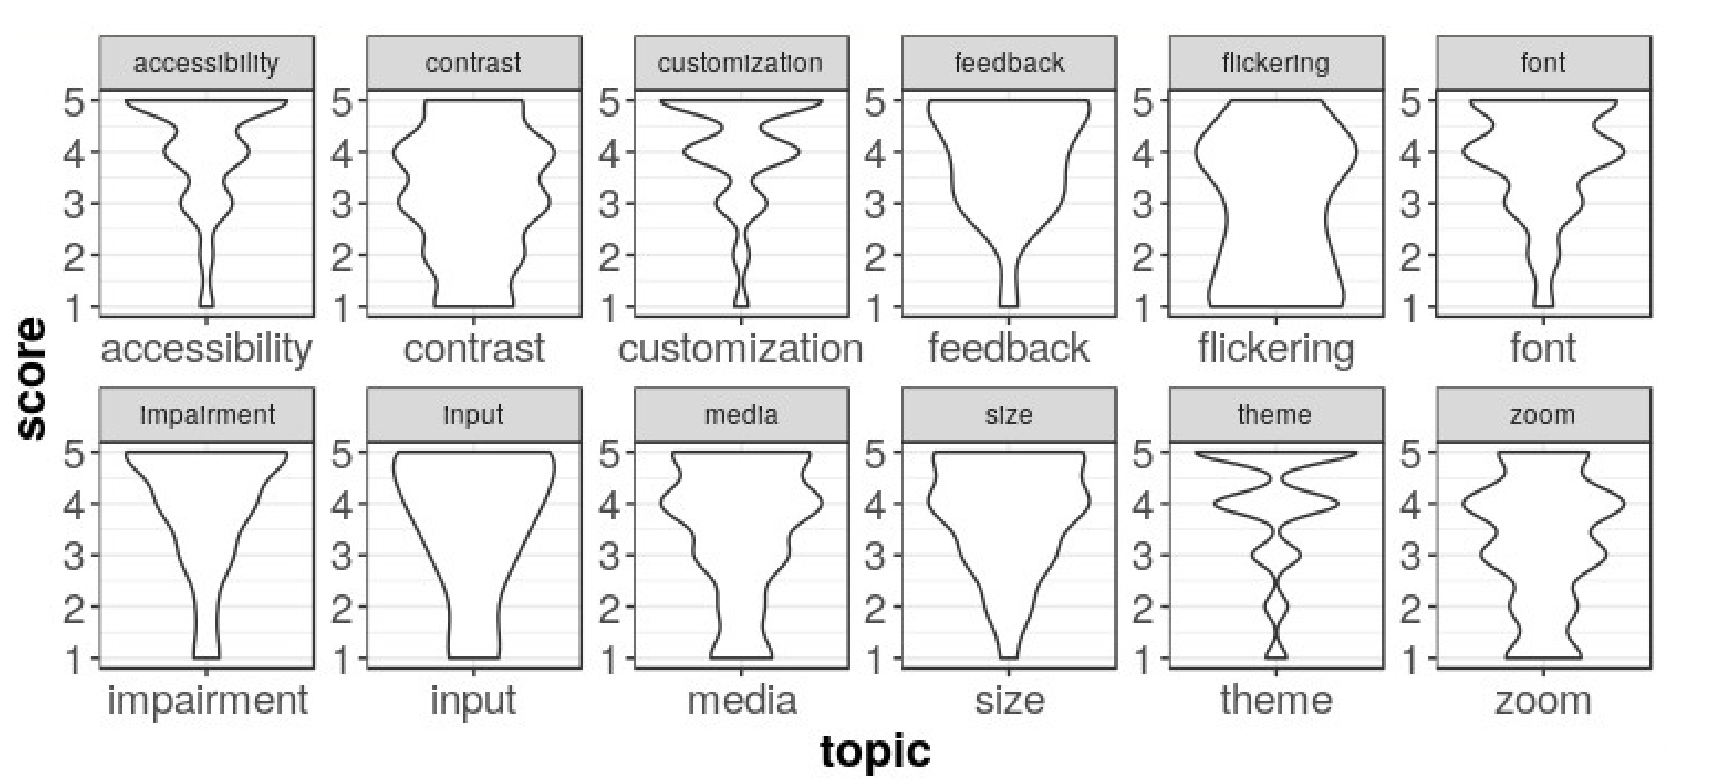
\includegraphics[scale=0.57]{imagens/score-themes-adapt.pdf}
\caption{Scores associated with the reviews that address an accessibility topic (cf. \autoref{tab:group-keywords})}
\label{fig:scoresthemes}
\end{figure*}

 \begin{figure*}[!htb]
 \centering
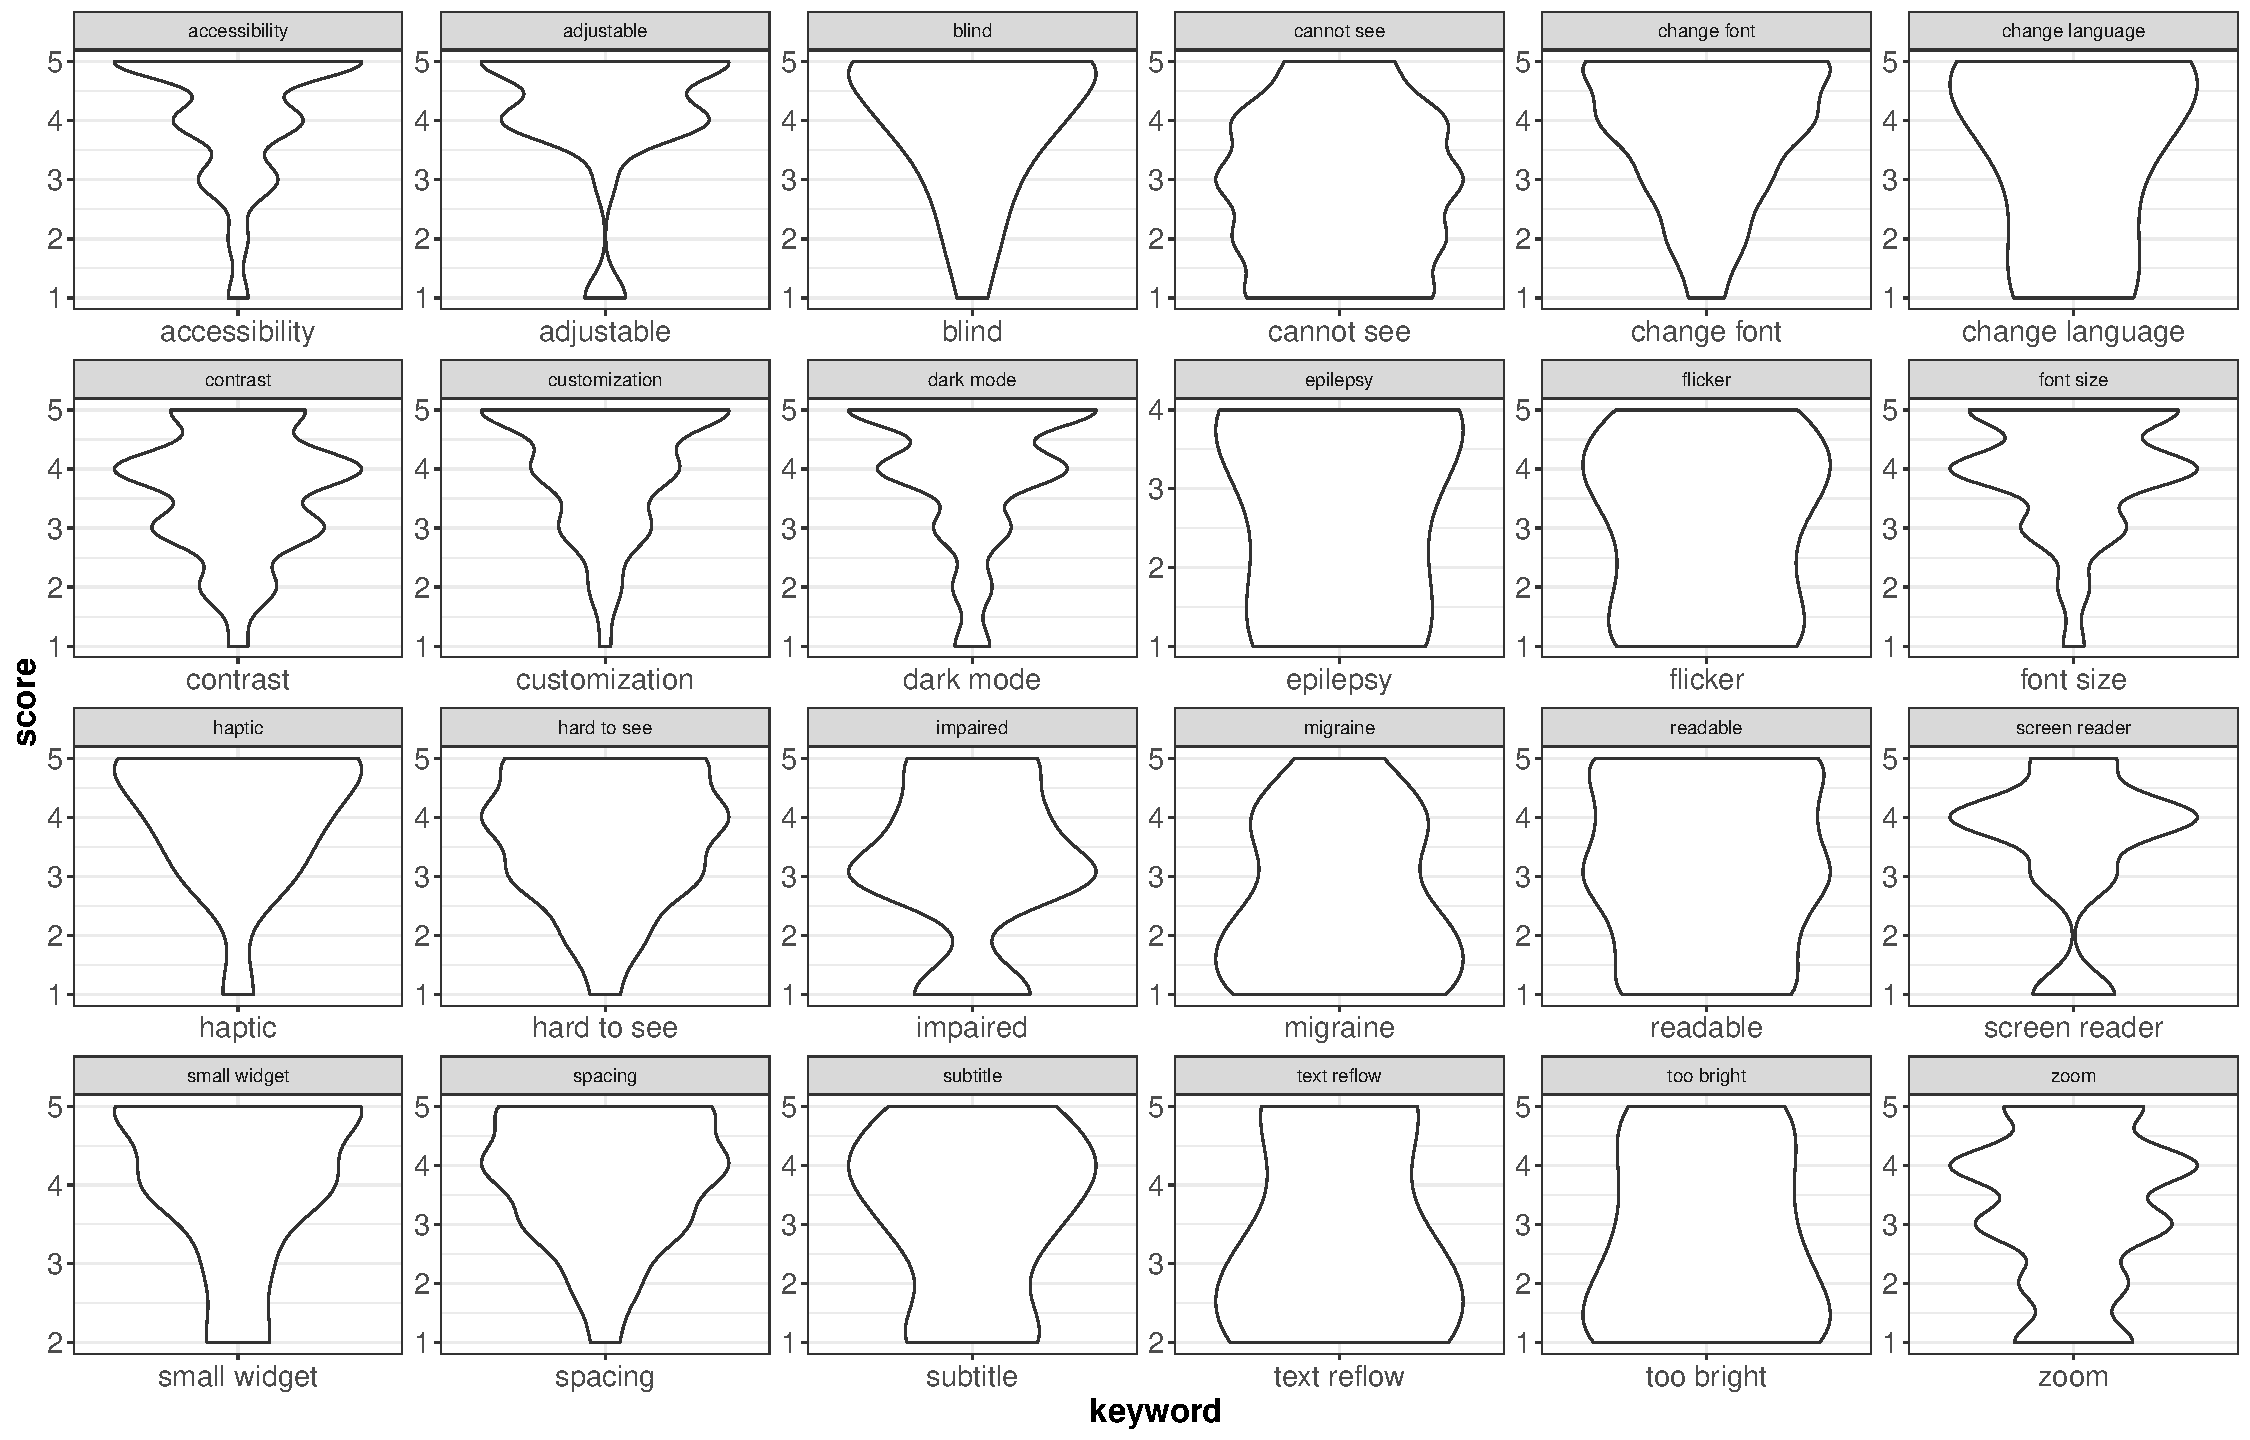
\includegraphics[scale=0.42]{imagens/keywords-scores.pdf}
\caption{Scores associated with the reviews that present a particular keyword}
\label{fig:scoreskeys}
\end{figure*}

\autoref{fig:scoreskeys} shows violin plots of the scores given by users to accessibility reviews that contain specific keywords. We do not show scores for all keywords due to space limitations. 
For some keywords, the scores are concentrated on the upper score level. This is the case of ``accessibility'', ``blind'', ``change font'', ``dark mode'', ``customization'', ``haptic'', and so forth. 
For others, there is a significant number of reviews with lower scores, such as in ``cannot see'', ``epilepsy'', ``flicker'', ``migraine'', ``readable'', ``text reflow'', and ``too bright''. This makes sense once the issues reported on reviews associated with such keywords are real barriers faced by users. Here are some examples of reviews that contain some of these keywords:
\begin{itemize}
 \item \textit{``Very little contrast. Bad for old eyes.''}
 \item \textit{``Wish it also handled older open doc formats - and that it would reflow text on zoom''}
 \item \textit{`` The flashing backgrounds could trigger an epilepsy and migraine''}
 \item \textit{``It's ok but the editing icons come up in white over the image.. which obviously means if you have a white image you cannot see them. Seriously - how could a developer get something so obvious that wrong? ''}
 \item \textit{`` Widget Text color is black. Unreadable''}
 \item \textit{``Too bright now on this update now. Can you option to inverted color? (black instead of white). Going to have to uninstall. Sorry.''}  
\end{itemize}

%Analyse reviews with the lowest scores (score == 1)


